\documentclass[1p]{elsarticle_modified}
%\bibliographystyle{elsarticle-num}

%\usepackage[colorlinks]{hyperref}
%\usepackage{abbrmath_seonhwa} %\Abb, \Ascr, \Acal ,\Abf, \Afrak
\usepackage{amsfonts}
\usepackage{amssymb}
\usepackage{amsmath}
\usepackage{amsthm}
\usepackage{scalefnt}
\usepackage{amsbsy}
\usepackage{kotex}
\usepackage{caption}
\usepackage{subfig}
\usepackage{color}
\usepackage{graphicx}
\usepackage{xcolor} %% white, black, red, green, blue, cyan, magenta, yellow
\usepackage{float}
\usepackage{setspace}
\usepackage{hyperref}

\usepackage{tikz}
\usetikzlibrary{arrows}

\usepackage{multirow}
\usepackage{array} % fixed length table
\usepackage{hhline}

%%%%%%%%%%%%%%%%%%%%%
\makeatletter
\renewcommand*\env@matrix[1][\arraystretch]{%
	\edef\arraystretch{#1}%
	\hskip -\arraycolsep
	\let\@ifnextchar\new@ifnextchar
	\array{*\c@MaxMatrixCols c}}
\makeatother %https://tex.stackexchange.com/questions/14071/how-can-i-increase-the-line-spacing-in-a-matrix
%%%%%%%%%%%%%%%

\usepackage[normalem]{ulem}

\newcommand{\msout}[1]{\ifmmode\text{\sout{\ensuremath{#1}}}\else\sout{#1}\fi}
%SOURCE: \msout is \stkout macro in https://tex.stackexchange.com/questions/20609/strikeout-in-math-mode

\newcommand{\cancel}[1]{
	\ifmmode
	{\color{red}\msout{#1}}
	\else
	{\color{red}\sout{#1}}
	\fi
}

\newcommand{\add}[1]{
	{\color{blue}\uwave{#1}}
}

\newcommand{\replace}[2]{
	\ifmmode
	{\color{red}\msout{#1}}{\color{blue}\uwave{#2}}
	\else
	{\color{red}\sout{#1}}{\color{blue}\uwave{#2}}
	\fi
}

\newcommand{\Sol}{\mathcal{S}} %segment
\newcommand{\D}{D} %diagram
\newcommand{\A}{\mathcal{A}} %arc


%%%%%%%%%%%%%%%%%%%%%%%%%%%%%5 test

\def\sl{\operatorname{\textup{SL}}(2,\Cbb)}
\def\psl{\operatorname{\textup{PSL}}(2,\Cbb)}
\def\quan{\mkern 1mu \triangleright \mkern 1mu}

\theoremstyle{definition}
\newtheorem{thm}{Theorem}[section]
\newtheorem{prop}[thm]{Proposition}
\newtheorem{lem}[thm]{Lemma}
\newtheorem{ques}[thm]{Question}
\newtheorem{cor}[thm]{Corollary}
\newtheorem{defn}[thm]{Definition}
\newtheorem{exam}[thm]{Example}
\newtheorem{rmk}[thm]{Remark}
\newtheorem{alg}[thm]{Algorithm}

\newcommand{\I}{\sqrt{-1}}
\begin{document}

%\begin{frontmatter}
%
%\title{Boundary parabolic representations of knots up to 8 crossings}
%
%%% Group authors per affiliation:
%\author{Yunhi Cho} 
%\address{Department of Mathematics, University of Seoul, Seoul, Korea}
%\ead{yhcho@uos.ac.kr}
%
%
%\author{Seonhwa Kim} %\fnref{s_kim}}
%\address{Center for Geometry and Physics, Institute for Basic Science, Pohang, 37673, Korea}
%\ead{ryeona17@ibs.re.kr}
%
%\author{Hyuk Kim}
%\address{Department of Mathematical Sciences, Seoul National University, Seoul 08826, Korea}
%\ead{hyukkim@snu.ac.kr}
%
%\author{Seokbeom Yoon}
%\address{Department of Mathematical Sciences, Seoul National University, Seoul, 08826,  Korea}
%\ead{sbyoon15@snu.ac.kr}
%
%\begin{abstract}
%We find all boundary parabolic representation of knots up to 8 crossings.
%
%\end{abstract}
%\begin{keyword}
%    \MSC[2010] 57M25 
%\end{keyword}
%
%\end{frontmatter}

%\linenumbers
%\tableofcontents
%
\newcommand\colored[1]{\textcolor{white}{\rule[-0.35ex]{0.8em}{1.4ex}}\kern-0.8em\color{red} #1}%
%\newcommand\colored[1]{\textcolor{white}{ #1}\kern-2.17ex	\textcolor{white}{ #1}\kern-1.81ex	\textcolor{white}{ #1}\kern-2.15ex\color{red}#1	}

{\Large $\underline{12n_{0106}~(K12n_{0106})}$}

\setlength{\tabcolsep}{10pt}
\renewcommand{\arraystretch}{1.6}
\vspace{1cm}\begin{tabular}{m{100pt}>{\centering\arraybackslash}m{274pt}}
\multirow{5}{120pt}{
	\centering
	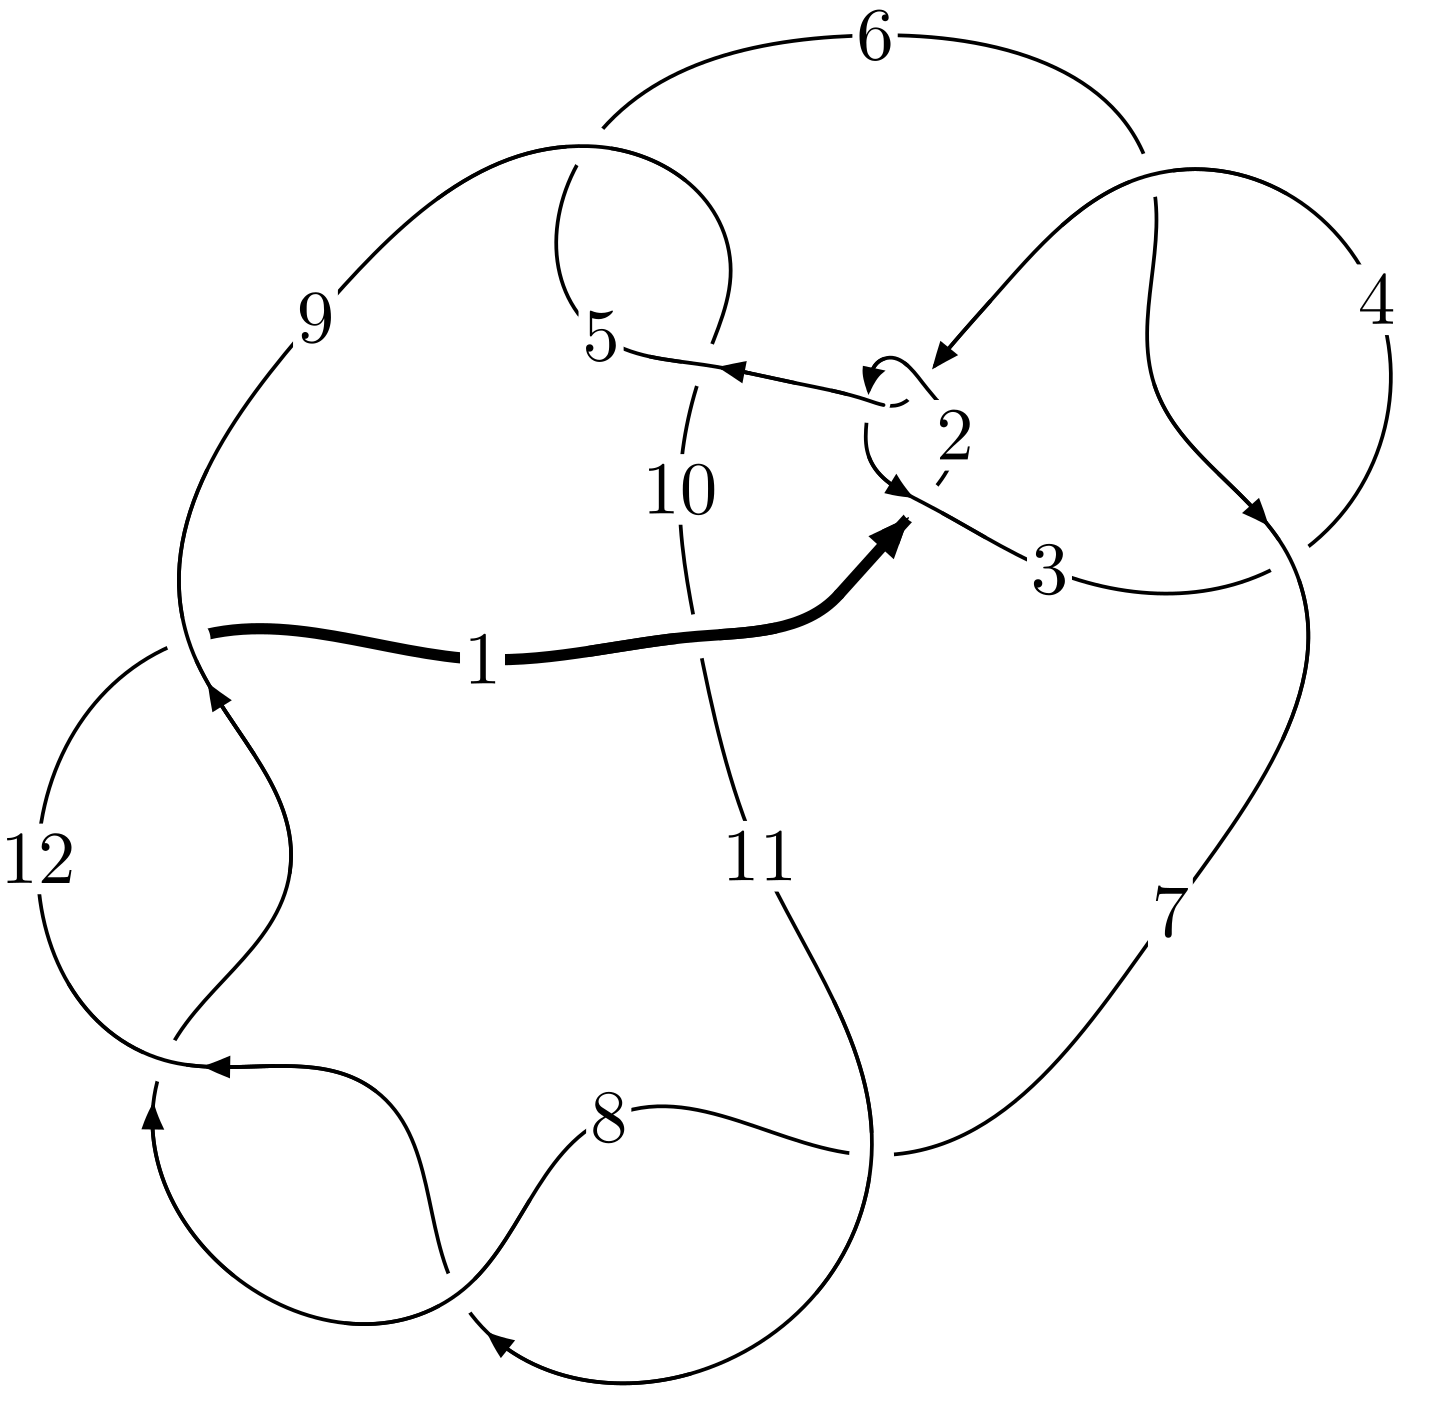
\includegraphics[width=112pt]{../../../GIT/diagram.site/Diagrams/png/2195_12n_0106.png}\\
\ \ \ A knot diagram\footnotemark}&
\allowdisplaybreaks
\textbf{Linearized knot diagam} \\
\cline{2-2}
 &
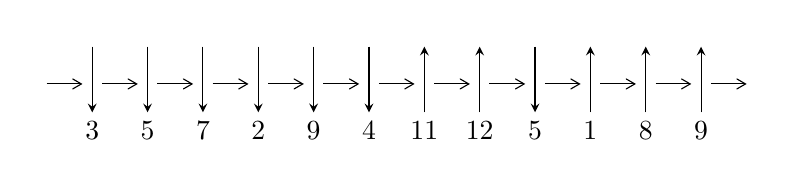
\begin{tikzpicture}[x=20pt, y=17pt]
	% nodes
	\node (C0) at (0, 0) {};
	\node (C1) at (1, 0) {};
	\node (C1U) at (1, +1) {};
	\node (C1D) at (1, -1) {3};

	\node (C2) at (2, 0) {};
	\node (C2U) at (2, +1) {};
	\node (C2D) at (2, -1) {5};

	\node (C3) at (3, 0) {};
	\node (C3U) at (3, +1) {};
	\node (C3D) at (3, -1) {7};

	\node (C4) at (4, 0) {};
	\node (C4U) at (4, +1) {};
	\node (C4D) at (4, -1) {2};

	\node (C5) at (5, 0) {};
	\node (C5U) at (5, +1) {};
	\node (C5D) at (5, -1) {9};

	\node (C6) at (6, 0) {};
	\node (C6U) at (6, +1) {};
	\node (C6D) at (6, -1) {4};

	\node (C7) at (7, 0) {};
	\node (C7U) at (7, +1) {};
	\node (C7D) at (7, -1) {11};

	\node (C8) at (8, 0) {};
	\node (C8U) at (8, +1) {};
	\node (C8D) at (8, -1) {12};

	\node (C9) at (9, 0) {};
	\node (C9U) at (9, +1) {};
	\node (C9D) at (9, -1) {5};

	\node (C10) at (10, 0) {};
	\node (C10U) at (10, +1) {};
	\node (C10D) at (10, -1) {1};

	\node (C11) at (11, 0) {};
	\node (C11U) at (11, +1) {};
	\node (C11D) at (11, -1) {8};

	\node (C12) at (12, 0) {};
	\node (C12U) at (12, +1) {};
	\node (C12D) at (12, -1) {9};
	\node (C13) at (13, 0) {};

	% arrows
	\draw[->,>={angle 60}]
	(C0) edge (C1) (C1) edge (C2) (C2) edge (C3) (C3) edge (C4) (C4) edge (C5) (C5) edge (C6) (C6) edge (C7) (C7) edge (C8) (C8) edge (C9) (C9) edge (C10) (C10) edge (C11) (C11) edge (C12) (C12) edge (C13) ;	\draw[->,>=stealth]
	(C1U) edge (C1D) (C2U) edge (C2D) (C3U) edge (C3D) (C4U) edge (C4D) (C5U) edge (C5D) (C6U) edge (C6D) (C7D) edge (C7U) (C8D) edge (C8U) (C9U) edge (C9D) (C10D) edge (C10U) (C11D) edge (C11U) (C12D) edge (C12U) ;
	\end{tikzpicture} \\
\hhline{~~} \\& 
\textbf{Solving Sequence} \\ \cline{2-2} 
 &
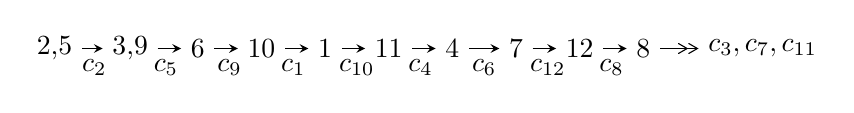
\begin{tikzpicture}[x=23pt, y=7pt]
	% node
	\node (A0) at (-1/8, 0) {2,5};
	\node (A1) at (17/16, 0) {3,9};
	\node (A2) at (17/8, 0) {6};
	\node (A3) at (25/8, 0) {10};
	\node (A4) at (33/8, 0) {1};
	\node (A5) at (41/8, 0) {11};
	\node (A6) at (49/8, 0) {4};
	\node (A7) at (57/8, 0) {7};
	\node (A8) at (65/8, 0) {12};
	\node (A9) at (73/8, 0) {8};
	\node (C1) at (1/2, -1) {$c_{2}$};
	\node (C2) at (13/8, -1) {$c_{5}$};
	\node (C3) at (21/8, -1) {$c_{9}$};
	\node (C4) at (29/8, -1) {$c_{1}$};
	\node (C5) at (37/8, -1) {$c_{10}$};
	\node (C6) at (45/8, -1) {$c_{4}$};
	\node (C7) at (53/8, -1) {$c_{6}$};
	\node (C8) at (61/8, -1) {$c_{12}$};
	\node (C9) at (69/8, -1) {$c_{8}$};
	\node (A10) at (11, 0) {$c_{3},c_{7},c_{11}$};

	% edge
	\draw[->,>=stealth]	
	(A0) edge (A1) (A1) edge (A2) (A2) edge (A3) (A3) edge (A4) (A4) edge (A5) (A5) edge (A6) (A6) edge (A7) (A7) edge (A8) (A8) edge (A9) ;
	\draw[->>,>={angle 60}]	
	(A9) edge (A10);
\end{tikzpicture} \\ 

\end{tabular} \\

\footnotetext{
The image of knot diagram is generated by the software ``\textbf{Draw programme}" developed by Andrew Bartholomew(\url{http://www.layer8.co.uk/maths/draw/index.htm\#Running-draw}), where we modified some parts for our purpose(\url{https://github.com/CATsTAILs/LinksPainter}).
}\phantom \\ \newline 
\centering \textbf{Ideals for irreducible components\footnotemark of $X_{\text{par}}$} 
 
\begin{align*}
I^u_{1}&=\langle 
2.95001\times10^{28} u^{46}+1.02756\times10^{29} u^{45}+\cdots+4.89243\times10^{27} b-4.24094\times10^{28},\\
\phantom{I^u_{1}}&\phantom{= \langle  }5.28780\times10^{28} u^{46}+1.85724\times10^{29} u^{45}+\cdots+2.44621\times10^{27} a-1.24073\times10^{29},\;u^{47}+4 u^{46}+\cdots-11 u-1\rangle \\
I^u_{2}&=\langle 
u^2 b+b^2+b u-2 u^2+b-3 u-2,\;a,\;u^3+u^2-1\rangle \\
I^u_{3}&=\langle 
b-2,\;a-1,\;u-1\rangle \\
\\
\end{align*}
\raggedright * 3 irreducible components of $\dim_{\mathbb{C}}=0$, with total 54 representations.\\
\footnotetext{All coefficients of polynomials are rational numbers. But the coefficients are sometimes approximated in decimal forms when there is not enough margin.}
\newpage
\renewcommand{\arraystretch}{1}
\centering \section*{I. $I^u_{1}= \langle 2.95\times10^{28} u^{46}+1.03\times10^{29} u^{45}+\cdots+4.89\times10^{27} b-4.24\times10^{28},\;5.29\times10^{28} u^{46}+1.86\times10^{29} u^{45}+\cdots+2.45\times10^{27} a-1.24\times10^{29},\;u^{47}+4 u^{46}+\cdots-11 u-1 \rangle$}
\flushleft \textbf{(i) Arc colorings}\\
\begin{tabular}{m{7pt} m{180pt} m{7pt} m{180pt} }
\flushright $a_{2}=$&$\begin{pmatrix}1\\0\end{pmatrix}$ \\
\flushright $a_{5}=$&$\begin{pmatrix}0\\u\end{pmatrix}$ \\
\flushright $a_{3}=$&$\begin{pmatrix}1\\u^2\end{pmatrix}$ \\
\flushright $a_{9}=$&$\begin{pmatrix}-21.6162 u^{46}-75.9230 u^{45}+\cdots+433.914 u+50.7202\\-6.02975 u^{46}-21.0031 u^{45}+\cdots+76.8942 u+8.66836\end{pmatrix}$ \\
\flushright $a_{6}=$&$\begin{pmatrix}29.5086 u^{46}+104.599 u^{45}+\cdots-601.499 u-73.1793\\11.4583 u^{46}+40.3975 u^{45}+\cdots-214.814 u-25.2675\end{pmatrix}$ \\
\flushright $a_{10}=$&$\begin{pmatrix}-21.6162 u^{46}-75.9230 u^{45}+\cdots+433.914 u+50.7202\\-12.4237 u^{46}-42.3264 u^{45}+\cdots+171.240 u+19.2103\end{pmatrix}$ \\
\flushright $a_{1}=$&$\begin{pmatrix}- u^2+1\\- u^4\end{pmatrix}$ \\
\flushright $a_{11}=$&$\begin{pmatrix}-26.2116 u^{46}-91.6779 u^{45}+\cdots+523.253 u+61.1104\\-10.1373 u^{46}-34.3085 u^{45}+\cdots+141.882 u+16.1328\end{pmatrix}$ \\
\flushright $a_{4}=$&$\begin{pmatrix}u\\u\end{pmatrix}$ \\
\flushright $a_{7}=$&$\begin{pmatrix}33.2674 u^{46}+117.852 u^{45}+\cdots-671.448 u-81.1792\\15.2170 u^{46}+53.6510 u^{45}+\cdots-284.762 u-33.2674\end{pmatrix}$ \\
\flushright $a_{12}=$&$\begin{pmatrix}23.3159 u^{46}+82.6280 u^{45}+\cdots-479.630 u-56.3099\\5.89371 u^{46}+20.0339 u^{45}+\cdots-139.693 u-15.9659\end{pmatrix}$ \\
\flushright $a_{8}=$&$\begin{pmatrix}2.05202 u^{46}+7.02641 u^{45}+\cdots-34.0094 u-5.57078\\5.07530 u^{46}+18.0511 u^{45}+\cdots-64.3990 u-8.02822\end{pmatrix}$\\&\end{tabular}
\flushleft \textbf{(ii) Obstruction class $= -1$}\\~\\
\flushleft \textbf{(iii) Cusp Shapes $= -19.4717 u^{46}-66.4148 u^{45}+\cdots+400.531 u+54.1723$}\\~\\
\newpage\renewcommand{\arraystretch}{1}
\flushleft \textbf{(iv) u-Polynomials at the component}\newline \\
\begin{tabular}{m{50pt}|m{274pt}}
Crossings & \hspace{64pt}u-Polynomials at each crossing \\
\hline $$\begin{aligned}c_{1}\end{aligned}$$&$\begin{aligned}
&u^{47}+26 u^{46}+\cdots+33 u+1
\end{aligned}$\\
\hline $$\begin{aligned}c_{2},c_{4}\end{aligned}$$&$\begin{aligned}
&u^{47}-4 u^{46}+\cdots-11 u+1
\end{aligned}$\\
\hline $$\begin{aligned}c_{3},c_{6}\end{aligned}$$&$\begin{aligned}
&u^{47}-3 u^{46}+\cdots-6 u+2
\end{aligned}$\\
\hline $$\begin{aligned}c_{5},c_{9}\end{aligned}$$&$\begin{aligned}
&u^{47}+2 u^{46}+\cdots-32 u-64
\end{aligned}$\\
\hline $$\begin{aligned}c_{7},c_{8},c_{11}\\c_{12}\end{aligned}$$&$\begin{aligned}
&u^{47}-5 u^{46}+\cdots-8 u-1
\end{aligned}$\\
\hline $$\begin{aligned}c_{10}\end{aligned}$$&$\begin{aligned}
&u^{47}+7 u^{46}+\cdots-5444 u+89
\end{aligned}$\\
\hline
\end{tabular}\\~\\
\newpage\renewcommand{\arraystretch}{1}
\flushleft \textbf{(v) Riley Polynomials at the component}\newline \\
\begin{tabular}{m{50pt}|m{274pt}}
Crossings & \hspace{64pt}Riley Polynomials at each crossing \\
\hline $$\begin{aligned}c_{1}\end{aligned}$$&$\begin{aligned}
&y^{47}-6 y^{46}+\cdots+193 y-1
\end{aligned}$\\
\hline $$\begin{aligned}c_{2},c_{4}\end{aligned}$$&$\begin{aligned}
&y^{47}-26 y^{46}+\cdots+33 y-1
\end{aligned}$\\
\hline $$\begin{aligned}c_{3},c_{6}\end{aligned}$$&$\begin{aligned}
&y^{47}+15 y^{46}+\cdots+315 y^2-4
\end{aligned}$\\
\hline $$\begin{aligned}c_{5},c_{9}\end{aligned}$$&$\begin{aligned}
&y^{47}-36 y^{46}+\cdots+168960 y-4096
\end{aligned}$\\
\hline $$\begin{aligned}c_{7},c_{8},c_{11}\\c_{12}\end{aligned}$$&$\begin{aligned}
&y^{47}-53 y^{46}+\cdots+138 y-1
\end{aligned}$\\
\hline $$\begin{aligned}c_{10}\end{aligned}$$&$\begin{aligned}
&y^{47}+31 y^{46}+\cdots+25436870 y-7921
\end{aligned}$\\
\hline
\end{tabular}\\~\\
\newpage\flushleft \textbf{(vi) Complex Volumes and Cusp Shapes}
$$\begin{array}{c|c|c}  
\text{Solutions to }I^u_{1}& \I (\text{vol} + \sqrt{-1}CS) & \text{Cusp shape}\\
 \hline 
\begin{aligned}
u &= \phantom{-}0.989960 + 0.148170 I \\
a &= \phantom{-}0.086218 + 0.547482 I \\
b &= \phantom{-}1.057400 - 0.538353 I\end{aligned}
 & -1.149640 - 0.628552 I & -5.94054 - 2.36276 I \\ \hline\begin{aligned}
u &= \phantom{-}0.989960 - 0.148170 I \\
a &= \phantom{-}0.086218 - 0.547482 I \\
b &= \phantom{-}1.057400 + 0.538353 I\end{aligned}
 & -1.149640 + 0.628552 I & -5.94054 + 2.36276 I \\ \hline\begin{aligned}
u &= -0.931667 + 0.360435 I \\
a &= \phantom{-}0.650552 - 1.137680 I \\
b &= \phantom{-}0.506455 - 0.859521 I\end{aligned}
 & \phantom{-}0.10041 + 3.44087 I & \phantom{-}0.17183 - 8.28941 I \\ \hline\begin{aligned}
u &= -0.931667 - 0.360435 I \\
a &= \phantom{-}0.650552 + 1.137680 I \\
b &= \phantom{-}0.506455 + 0.859521 I\end{aligned}
 & \phantom{-}0.10041 - 3.44087 I & \phantom{-}0.17183 + 8.28941 I \\ \hline\begin{aligned}
u &= -0.223147 + 1.003930 I \\
a &= -0.312504 + 1.368880 I \\
b &= -0.143382 - 0.236139 I\end{aligned}
 & \phantom{-}5.63196 - 8.09738 I & \phantom{-}3.35253 + 4.54237 I \\ \hline\begin{aligned}
u &= -0.223147 - 1.003930 I \\
a &= -0.312504 - 1.368880 I \\
b &= -0.143382 + 0.236139 I\end{aligned}
 & \phantom{-}5.63196 + 8.09738 I & \phantom{-}3.35253 - 4.54237 I \\ \hline\begin{aligned}
u &= \phantom{-}0.951382\phantom{ +0.000000I} \\
a &= -0.361021\phantom{ +0.000000I} \\
b &= -4.05034\phantom{ +0.000000I}\end{aligned}
 & -0.451802\phantom{ +0.000000I} & -56.4450\phantom{ +0.000000I} \\ \hline\begin{aligned}
u &= -0.108798 + 0.923471 I \\
a &= \phantom{-}0.29912 - 1.44151 I \\
b &= -0.019834 + 0.147643 I\end{aligned}
 & -1.70582 - 5.21126 I & \phantom{-}0.15580 + 5.73446 I \\ \hline\begin{aligned}
u &= -0.108798 - 0.923471 I \\
a &= \phantom{-}0.29912 + 1.44151 I \\
b &= -0.019834 - 0.147643 I\end{aligned}
 & -1.70582 + 5.21126 I & \phantom{-}0.15580 - 5.73446 I \\ \hline\begin{aligned}
u &= \phantom{-}0.375825 + 0.801282 I \\
a &= \phantom{-}0.38215 - 1.40610 I \\
b &= -0.312468 - 0.166120 I\end{aligned}
 & \phantom{-}3.28905 + 1.41624 I & \phantom{-}1.285372 - 0.077907 I\\
 \hline 
 \end{array}$$\newpage$$\begin{array}{c|c|c}  
\text{Solutions to }I^u_{1}& \I (\text{vol} + \sqrt{-1}CS) & \text{Cusp shape}\\
 \hline 
\begin{aligned}
u &= \phantom{-}0.375825 - 0.801282 I \\
a &= \phantom{-}0.38215 + 1.40610 I \\
b &= -0.312468 + 0.166120 I\end{aligned}
 & \phantom{-}3.28905 - 1.41624 I & \phantom{-}1.285372 + 0.077907 I \\ \hline\begin{aligned}
u &= -0.754499 + 0.439436 I \\
a &= \phantom{-}0.787718 + 0.900721 I \\
b &= \phantom{-}1.67009 - 0.64753 I\end{aligned}
 & \phantom{-}10.33830 + 1.89063 I & \phantom{-}3.79886 - 2.45073 I \\ \hline\begin{aligned}
u &= -0.754499 - 0.439436 I \\
a &= \phantom{-}0.787718 - 0.900721 I \\
b &= \phantom{-}1.67009 + 0.64753 I\end{aligned}
 & \phantom{-}10.33830 - 1.89063 I & \phantom{-}3.79886 + 2.45073 I \\ \hline\begin{aligned}
u &= \phantom{-}0.848625\phantom{ +0.000000I} \\
a &= \phantom{-}0.348245\phantom{ +0.000000I} \\
b &= \phantom{-}5.16287\phantom{ +0.000000I}\end{aligned}
 & \phantom{-}7.65141\phantom{ +0.000000I} & -49.4120\phantom{ +0.000000I} \\ \hline\begin{aligned}
u &= -0.874869 + 0.786950 I \\
a &= -0.309968 - 0.224071 I \\
b &= -0.262520 - 0.143001 I\end{aligned}
 & \phantom{-}3.72699 + 2.94871 I & -12.2330 - 7.8683 I \\ \hline\begin{aligned}
u &= -0.874869 - 0.786950 I \\
a &= -0.309968 + 0.224071 I \\
b &= -0.262520 + 0.143001 I\end{aligned}
 & \phantom{-}3.72699 - 2.94871 I & -12.2330 + 7.8683 I \\ \hline\begin{aligned}
u &= \phantom{-}1.126180 + 0.347504 I \\
a &= -0.188549 - 0.855543 I \\
b &= -1.147560 - 0.094454 I\end{aligned}
 & \phantom{-}5.11792 - 1.20868 I & \phantom{-0.000000 } 0 \\ \hline\begin{aligned}
u &= \phantom{-}1.126180 - 0.347504 I \\
a &= -0.188549 + 0.855543 I \\
b &= -1.147560 + 0.094454 I\end{aligned}
 & \phantom{-}5.11792 + 1.20868 I & \phantom{-0.000000 } 0 \\ \hline\begin{aligned}
u &= \phantom{-}0.059234 + 0.812807 I \\
a &= -0.34521 + 1.50868 I \\
b &= \phantom{-}0.186918 - 0.028378 I\end{aligned}
 & -2.49343 - 1.08855 I & -2.03214 + 0.04750 I \\ \hline\begin{aligned}
u &= \phantom{-}0.059234 - 0.812807 I \\
a &= -0.34521 - 1.50868 I \\
b &= \phantom{-}0.186918 + 0.028378 I\end{aligned}
 & -2.49343 + 1.08855 I & -2.03214 - 0.04750 I\\
 \hline 
 \end{array}$$\newpage$$\begin{array}{c|c|c}  
\text{Solutions to }I^u_{1}& \I (\text{vol} + \sqrt{-1}CS) & \text{Cusp shape}\\
 \hline 
\begin{aligned}
u &= -1.144920 + 0.321301 I \\
a &= -1.39264 - 0.30017 I \\
b &= -2.50504 + 0.05350 I\end{aligned}
 & -1.09956 + 1.43032 I & \phantom{-0.000000 } 0 \\ \hline\begin{aligned}
u &= -1.144920 - 0.321301 I \\
a &= -1.39264 + 0.30017 I \\
b &= -2.50504 - 0.05350 I\end{aligned}
 & -1.09956 - 1.43032 I & \phantom{-0.000000 } 0 \\ \hline\begin{aligned}
u &= -1.109420 + 0.477918 I \\
a &= -0.225844 + 1.135400 I \\
b &= -0.151788 + 0.912718 I\end{aligned}
 & \phantom{-}6.07282 + 6.30143 I & \phantom{-0.000000 } 0 \\ \hline\begin{aligned}
u &= -1.109420 - 0.477918 I \\
a &= -0.225844 - 1.135400 I \\
b &= -0.151788 - 0.912718 I\end{aligned}
 & \phantom{-}6.07282 - 6.30143 I & \phantom{-0.000000 } 0 \\ \hline\begin{aligned}
u &= -0.889179 + 0.911068 I \\
a &= \phantom{-}0.567632 + 0.472874 I \\
b &= \phantom{-}0.506073 + 0.310758 I\end{aligned}
 & \phantom{-}10.50090 + 3.30217 I & \phantom{-0.000000 } 0 \\ \hline\begin{aligned}
u &= -0.889179 - 0.911068 I \\
a &= \phantom{-}0.567632 - 0.472874 I \\
b &= \phantom{-}0.506073 - 0.310758 I\end{aligned}
 & \phantom{-}10.50090 - 3.30217 I & \phantom{-0.000000 } 0 \\ \hline\begin{aligned}
u &= \phantom{-}1.157290 + 0.591284 I \\
a &= \phantom{-}1.109010 - 0.155564 I \\
b &= \phantom{-}2.14720 - 0.71964 I\end{aligned}
 & \phantom{-}0.92342 - 6.68779 I & \phantom{-0.000000 } 0 \\ \hline\begin{aligned}
u &= \phantom{-}1.157290 - 0.591284 I \\
a &= \phantom{-}1.109010 + 0.155564 I \\
b &= \phantom{-}2.14720 + 0.71964 I\end{aligned}
 & \phantom{-}0.92342 + 6.68779 I & \phantom{-0.000000 } 0 \\ \hline\begin{aligned}
u &= -1.230280 + 0.438166 I \\
a &= \phantom{-}1.292840 + 0.114739 I \\
b &= \phantom{-}2.59516 - 0.07060 I\end{aligned}
 & -6.29518 + 5.50452 I & \phantom{-0.000000 } 0 \\ \hline\begin{aligned}
u &= -1.230280 - 0.438166 I \\
a &= \phantom{-}1.292840 - 0.114739 I \\
b &= \phantom{-}2.59516 + 0.07060 I\end{aligned}
 & -6.29518 - 5.50452 I & \phantom{-0.000000 } 0\\
 \hline 
 \end{array}$$\newpage$$\begin{array}{c|c|c}  
\text{Solutions to }I^u_{1}& \I (\text{vol} + \sqrt{-1}CS) & \text{Cusp shape}\\
 \hline 
\begin{aligned}
u &= \phantom{-}1.221460 + 0.493956 I \\
a &= -1.035260 + 0.239047 I \\
b &= -2.17910 + 0.67973 I\end{aligned}
 & -5.89684 - 3.67490 I & \phantom{-0.000000 } 0 \\ \hline\begin{aligned}
u &= \phantom{-}1.221460 - 0.493956 I \\
a &= -1.035260 - 0.239047 I \\
b &= -2.17910 - 0.67973 I\end{aligned}
 & -5.89684 + 3.67490 I & \phantom{-0.000000 } 0 \\ \hline\begin{aligned}
u &= \phantom{-}0.669427\phantom{ +0.000000I} \\
a &= -0.452367\phantom{ +0.000000I} \\
b &= \phantom{-}0.335316\phantom{ +0.000000I}\end{aligned}
 & -1.01372\phantom{ +0.000000I} & -10.3930\phantom{ +0.000000I} \\ \hline\begin{aligned}
u &= -0.178892 + 0.636081 I \\
a &= \phantom{-}1.61229 + 0.11889 I \\
b &= \phantom{-}0.969029 - 0.433870 I\end{aligned}
 & \phantom{-}8.67414 - 2.02923 I & \phantom{-}6.38070 + 1.31837 I \\ \hline\begin{aligned}
u &= -0.178892 - 0.636081 I \\
a &= \phantom{-}1.61229 - 0.11889 I \\
b &= \phantom{-}0.969029 + 0.433870 I\end{aligned}
 & \phantom{-}8.67414 + 2.02923 I & \phantom{-}6.38070 - 1.31837 I \\ \hline\begin{aligned}
u &= \phantom{-}1.286390 + 0.397327 I \\
a &= \phantom{-}0.966983 - 0.333762 I \\
b &= \phantom{-}2.17649 - 0.61779 I\end{aligned}
 & -6.10647 + 0.63964 I & \phantom{-0.000000 } 0 \\ \hline\begin{aligned}
u &= \phantom{-}1.286390 - 0.397327 I \\
a &= \phantom{-}0.966983 + 0.333762 I \\
b &= \phantom{-}2.17649 + 0.61779 I\end{aligned}
 & -6.10647 - 0.63964 I & \phantom{-0.000000 } 0 \\ \hline\begin{aligned}
u &= -1.251910 + 0.523865 I \\
a &= -1.226570 - 0.021764 I \\
b &= -2.63642 + 0.05168 I\end{aligned}
 & -5.19394 + 10.42330 I & \phantom{-0.000000 } 0 \\ \hline\begin{aligned}
u &= -1.251910 - 0.523865 I \\
a &= -1.226570 + 0.021764 I \\
b &= -2.63642 - 0.05168 I\end{aligned}
 & -5.19394 - 10.42330 I & \phantom{-0.000000 } 0 \\ \hline\begin{aligned}
u &= -1.252930 + 0.595086 I \\
a &= \phantom{-}1.168960 - 0.050135 I \\
b &= \phantom{-}2.66504 - 0.01710 I\end{aligned}
 & \phantom{-}2.45160 + 13.84790 I & \phantom{-0.000000 } 0\\
 \hline 
 \end{array}$$\newpage$$\begin{array}{c|c|c}  
\text{Solutions to }I^u_{1}& \I (\text{vol} + \sqrt{-1}CS) & \text{Cusp shape}\\
 \hline 
\begin{aligned}
u &= -1.252930 - 0.595086 I \\
a &= \phantom{-}1.168960 + 0.050135 I \\
b &= \phantom{-}2.66504 + 0.01710 I\end{aligned}
 & \phantom{-}2.45160 - 13.84790 I & \phantom{-0.000000 } 0 \\ \hline\begin{aligned}
u &= \phantom{-}1.366130 + 0.294990 I \\
a &= -0.908758 + 0.454189 I \\
b &= -2.11656 + 0.55334 I\end{aligned}
 & \phantom{-}0.27703 + 3.60334 I & \phantom{-0.000000 } 0 \\ \hline\begin{aligned}
u &= \phantom{-}1.366130 - 0.294990 I \\
a &= -0.908758 - 0.454189 I \\
b &= -2.11656 - 0.55334 I\end{aligned}
 & \phantom{-}0.27703 - 3.60334 I & \phantom{-0.000000 } 0 \\ \hline\begin{aligned}
u &= -0.591311 + 0.089878 I \\
a &= -1.40817 + 1.26783 I \\
b &= -0.997142 + 0.442455 I\end{aligned}
 & \phantom{-}1.303350 - 0.477077 I & \phantom{-}6.44413 + 0.83351 I \\ \hline\begin{aligned}
u &= -0.591311 - 0.089878 I \\
a &= -1.40817 - 1.26783 I \\
b &= -0.997142 - 0.442455 I\end{aligned}
 & \phantom{-}1.303350 + 0.477077 I & \phantom{-}6.44413 - 0.83351 I \\ \hline\begin{aligned}
u &= -0.275356 + 0.071579 I \\
a &= -2.33744 + 1.67178 I \\
b &= -0.731969 + 0.318628 I\end{aligned}
 & \phantom{-}1.33872 - 0.48836 I & \phantom{-}6.23098 + 1.53144 I \\ \hline\begin{aligned}
u &= -0.275356 - 0.071579 I \\
a &= -2.33744 - 1.67178 I \\
b &= -0.731969 - 0.318628 I\end{aligned}
 & \phantom{-}1.33872 + 0.48836 I & \phantom{-}6.23098 - 1.53144 I\\
 \hline 
 \end{array}$$\newpage\newpage\renewcommand{\arraystretch}{1}
\centering \section*{II. $I^u_{2}= \langle u^2 b+b^2+b u-2 u^2+b-3 u-2,\;a,\;u^3+u^2-1 \rangle$}
\flushleft \textbf{(i) Arc colorings}\\
\begin{tabular}{m{7pt} m{180pt} m{7pt} m{180pt} }
\flushright $a_{2}=$&$\begin{pmatrix}1\\0\end{pmatrix}$ \\
\flushright $a_{5}=$&$\begin{pmatrix}0\\u\end{pmatrix}$ \\
\flushright $a_{3}=$&$\begin{pmatrix}1\\u^2\end{pmatrix}$ \\
\flushright $a_{9}=$&$\begin{pmatrix}0\\b\end{pmatrix}$ \\
\flushright $a_{6}=$&$\begin{pmatrix}0\\u\end{pmatrix}$ \\
\flushright $a_{10}=$&$\begin{pmatrix}0\\b\end{pmatrix}$ \\
\flushright $a_{1}=$&$\begin{pmatrix}- u^2+1\\- u^2- u+1\end{pmatrix}$ \\
\flushright $a_{11}=$&$\begin{pmatrix}- u^2 b+b u\\-2 u^2 b+2 b\end{pmatrix}$ \\
\flushright $a_{4}=$&$\begin{pmatrix}u\\u\end{pmatrix}$ \\
\flushright $a_{7}=$&$\begin{pmatrix}u^2-1\\u^2+u-1\end{pmatrix}$ \\
\flushright $a_{12}=$&$\begin{pmatrix}- u^2+1\\- b+2\end{pmatrix}$ \\
\flushright $a_{8}=$&$\begin{pmatrix}u^2 b- b u\\2 u^2 b+u^2-2 b+u+1\end{pmatrix}$\\&\end{tabular}
\flushleft \textbf{(ii) Obstruction class $= 1$}\\~\\
\flushleft \textbf{(iii) Cusp Shapes $= -4 u^2 b- b u- u^2- b- u+10$}\\~\\
\newpage\renewcommand{\arraystretch}{1}
\flushleft \textbf{(iv) u-Polynomials at the component}\newline \\
\begin{tabular}{m{50pt}|m{274pt}}
Crossings & \hspace{64pt}u-Polynomials at each crossing \\
\hline $$\begin{aligned}c_{1},c_{3}\end{aligned}$$&$\begin{aligned}
&(u^3- u^2+2 u-1)^2
\end{aligned}$\\
\hline $$\begin{aligned}c_{2}\end{aligned}$$&$\begin{aligned}
&(u^3+u^2-1)^2
\end{aligned}$\\
\hline $$\begin{aligned}c_{4}\end{aligned}$$&$\begin{aligned}
&(u^3- u^2+1)^2
\end{aligned}$\\
\hline $$\begin{aligned}c_{5},c_{9}\end{aligned}$$&$\begin{aligned}
&u^6
\end{aligned}$\\
\hline $$\begin{aligned}c_{6}\end{aligned}$$&$\begin{aligned}
&(u^3+u^2+2 u+1)^2
\end{aligned}$\\
\hline $$\begin{aligned}c_{7},c_{8},c_{10}\end{aligned}$$&$\begin{aligned}
&(u^2- u-1)^3
\end{aligned}$\\
\hline $$\begin{aligned}c_{11},c_{12}\end{aligned}$$&$\begin{aligned}
&(u^2+u-1)^3
\end{aligned}$\\
\hline
\end{tabular}\\~\\
\newpage\renewcommand{\arraystretch}{1}
\flushleft \textbf{(v) Riley Polynomials at the component}\newline \\
\begin{tabular}{m{50pt}|m{274pt}}
Crossings & \hspace{64pt}Riley Polynomials at each crossing \\
\hline $$\begin{aligned}c_{1},c_{3},c_{6}\end{aligned}$$&$\begin{aligned}
&(y^3+3 y^2+2 y-1)^2
\end{aligned}$\\
\hline $$\begin{aligned}c_{2},c_{4}\end{aligned}$$&$\begin{aligned}
&(y^3- y^2+2 y-1)^2
\end{aligned}$\\
\hline $$\begin{aligned}c_{5},c_{9}\end{aligned}$$&$\begin{aligned}
&y^6
\end{aligned}$\\
\hline $$\begin{aligned}c_{7},c_{8},c_{10}\\c_{11},c_{12}\end{aligned}$$&$\begin{aligned}
&(y^2-3 y+1)^3
\end{aligned}$\\
\hline
\end{tabular}\\~\\
\newpage\flushleft \textbf{(vi) Complex Volumes and Cusp Shapes}
$$\begin{array}{c|c|c}  
\text{Solutions to }I^u_{2}& \I (\text{vol} + \sqrt{-1}CS) & \text{Cusp shape}\\
 \hline 
\begin{aligned}
u &= -0.877439 + 0.744862 I \\
a &= \phantom{-0.000000 } 0 \\
b &= -0.546315 + 0.909787 I\end{aligned}
 & \phantom{-}11.90680 + 2.82812 I & \phantom{-}7.12010 - 2.78145 I \\ \hline\begin{aligned}
u &= -0.877439 + 0.744862 I \\
a &= \phantom{-0.000000 } 0 \\
b &= \phantom{-}0.208674 - 0.347508 I\end{aligned}
 & \phantom{-}4.01109 + 2.82812 I & \phantom{-}12.01538 + 1.83947 I \\ \hline\begin{aligned}
u &= -0.877439 - 0.744862 I \\
a &= \phantom{-0.000000 } 0 \\
b &= -0.546315 - 0.909787 I\end{aligned}
 & \phantom{-}11.90680 - 2.82812 I & \phantom{-}7.12010 + 2.78145 I \\ \hline\begin{aligned}
u &= -0.877439 - 0.744862 I \\
a &= \phantom{-0.000000 } 0 \\
b &= \phantom{-}0.208674 + 0.347508 I\end{aligned}
 & \phantom{-}4.01109 - 2.82812 I & \phantom{-}12.01538 - 1.83947 I \\ \hline\begin{aligned}
u &= \phantom{-}0.754878\phantom{ +0.000000I} \\
a &= \phantom{-0.000000 } 0 \\
b &= \phantom{-}1.43675\phantom{ +0.000000I}\end{aligned}
 & -0.126494\phantom{ +0.000000I} & \phantom{-}2.87910\phantom{ +0.000000I} \\ \hline\begin{aligned}
u &= \phantom{-}0.754878\phantom{ +0.000000I} \\
a &= \phantom{-0.000000 } 0 \\
b &= -3.76147\phantom{ +0.000000I}\end{aligned}
 & \phantom{-}7.76919\phantom{ +0.000000I} & \phantom{-}23.8500\phantom{ +0.000000I}\\
 \hline 
 \end{array}$$\newpage\newpage\renewcommand{\arraystretch}{1}
\centering \section*{III. $I^u_{3}= \langle b-2,\;a-1,\;u-1 \rangle$}
\flushleft \textbf{(i) Arc colorings}\\
\begin{tabular}{m{7pt} m{180pt} m{7pt} m{180pt} }
\flushright $a_{2}=$&$\begin{pmatrix}1\\0\end{pmatrix}$ \\
\flushright $a_{5}=$&$\begin{pmatrix}0\\1\end{pmatrix}$ \\
\flushright $a_{3}=$&$\begin{pmatrix}1\\1\end{pmatrix}$ \\
\flushright $a_{9}=$&$\begin{pmatrix}1\\2\end{pmatrix}$ \\
\flushright $a_{6}=$&$\begin{pmatrix}-1\\-1\end{pmatrix}$ \\
\flushright $a_{10}=$&$\begin{pmatrix}1\\3\end{pmatrix}$ \\
\flushright $a_{1}=$&$\begin{pmatrix}0\\-1\end{pmatrix}$ \\
\flushright $a_{11}=$&$\begin{pmatrix}1\\2\end{pmatrix}$ \\
\flushright $a_{4}=$&$\begin{pmatrix}1\\1\end{pmatrix}$ \\
\flushright $a_{7}=$&$\begin{pmatrix}-1\\-1\end{pmatrix}$ \\
\flushright $a_{12}=$&$\begin{pmatrix}1\\1\end{pmatrix}$ \\
\flushright $a_{8}=$&$\begin{pmatrix}0\\1\end{pmatrix}$\\&\end{tabular}
\flushleft \textbf{(ii) Obstruction class $= 1$}\\~\\
\flushleft \textbf{(iii) Cusp Shapes $= 0$}\\~\\
\newpage\renewcommand{\arraystretch}{1}
\flushleft \textbf{(iv) u-Polynomials at the component}\newline \\
\begin{tabular}{m{50pt}|m{274pt}}
Crossings & \hspace{64pt}u-Polynomials at each crossing \\
\hline $$\begin{aligned}c_{1},c_{2},c_{9}\\c_{11},c_{12}\end{aligned}$$&$\begin{aligned}
&u-1
\end{aligned}$\\
\hline $$\begin{aligned}c_{3},c_{6}\end{aligned}$$&$\begin{aligned}
&u
\end{aligned}$\\
\hline $$\begin{aligned}c_{4},c_{5},c_{7}\\c_{8},c_{10}\end{aligned}$$&$\begin{aligned}
&u+1
\end{aligned}$\\
\hline
\end{tabular}\\~\\
\newpage\renewcommand{\arraystretch}{1}
\flushleft \textbf{(v) Riley Polynomials at the component}\newline \\
\begin{tabular}{m{50pt}|m{274pt}}
Crossings & \hspace{64pt}Riley Polynomials at each crossing \\
\hline $$\begin{aligned}c_{1},c_{2},c_{4}\\c_{5},c_{7},c_{8}\\c_{9},c_{10},c_{11}\\c_{12}\end{aligned}$$&$\begin{aligned}
&y-1
\end{aligned}$\\
\hline $$\begin{aligned}c_{3},c_{6}\end{aligned}$$&$\begin{aligned}
&y
\end{aligned}$\\
\hline
\end{tabular}\\~\\
\newpage\flushleft \textbf{(vi) Complex Volumes and Cusp Shapes}
$$\begin{array}{c|c|c}  
\text{Solutions to }I^u_{3}& \I (\text{vol} + \sqrt{-1}CS) & \text{Cusp shape}\\
 \hline 
\begin{aligned}
u &= \phantom{-}1.00000\phantom{ +0.000000I} \\
a &= \phantom{-}1.00000\phantom{ +0.000000I} \\
b &= \phantom{-}2.00000\phantom{ +0.000000I}\end{aligned}
 & \phantom{-0.000000 } 0 & \phantom{-0.000000 } 0\\
 \hline 
 \end{array}$$\newpage
\newpage\renewcommand{\arraystretch}{1}
\centering \section*{ IV. u-Polynomials}
\begin{tabular}{m{50pt}|m{274pt}}
Crossings & \hspace{64pt}u-Polynomials at each crossing \\
\hline $$\begin{aligned}c_{1}\end{aligned}$$&$\begin{aligned}
&(u-1)(u^3- u^2+2 u-1)^2(u^{47}+26 u^{46}+\cdots+33 u+1)
\end{aligned}$\\
\hline $$\begin{aligned}c_{2}\end{aligned}$$&$\begin{aligned}
&(u-1)(u^3+u^2-1)^2(u^{47}-4 u^{46}+\cdots-11 u+1)
\end{aligned}$\\
\hline $$\begin{aligned}c_{3}\end{aligned}$$&$\begin{aligned}
&u(u^3- u^2+2 u-1)^2(u^{47}-3 u^{46}+\cdots-6 u+2)
\end{aligned}$\\
\hline $$\begin{aligned}c_{4}\end{aligned}$$&$\begin{aligned}
&(u+1)(u^3- u^2+1)^2(u^{47}-4 u^{46}+\cdots-11 u+1)
\end{aligned}$\\
\hline $$\begin{aligned}c_{5}\end{aligned}$$&$\begin{aligned}
&u^6(u+1)(u^{47}+2 u^{46}+\cdots-32 u-64)
\end{aligned}$\\
\hline $$\begin{aligned}c_{6}\end{aligned}$$&$\begin{aligned}
&u(u^3+u^2+2 u+1)^2(u^{47}-3 u^{46}+\cdots-6 u+2)
\end{aligned}$\\
\hline $$\begin{aligned}c_{7},c_{8}\end{aligned}$$&$\begin{aligned}
&(u+1)(u^2- u-1)^3(u^{47}-5 u^{46}+\cdots-8 u-1)
\end{aligned}$\\
\hline $$\begin{aligned}c_{9}\end{aligned}$$&$\begin{aligned}
&u^6(u-1)(u^{47}+2 u^{46}+\cdots-32 u-64)
\end{aligned}$\\
\hline $$\begin{aligned}c_{10}\end{aligned}$$&$\begin{aligned}
&(u+1)(u^2- u-1)^3(u^{47}+7 u^{46}+\cdots-5444 u+89)
\end{aligned}$\\
\hline $$\begin{aligned}c_{11},c_{12}\end{aligned}$$&$\begin{aligned}
&(u-1)(u^2+u-1)^3(u^{47}-5 u^{46}+\cdots-8 u-1)
\end{aligned}$\\
\hline
\end{tabular}\newpage\renewcommand{\arraystretch}{1}
\centering \section*{ V. Riley Polynomials}
\begin{tabular}{m{50pt}|m{274pt}}
Crossings & \hspace{64pt}Riley Polynomials at each crossing \\
\hline $$\begin{aligned}c_{1}\end{aligned}$$&$\begin{aligned}
&(y-1)(y^3+3 y^2+2 y-1)^2(y^{47}-6 y^{46}+\cdots+193 y-1)
\end{aligned}$\\
\hline $$\begin{aligned}c_{2},c_{4}\end{aligned}$$&$\begin{aligned}
&(y-1)(y^3- y^2+2 y-1)^2(y^{47}-26 y^{46}+\cdots+33 y-1)
\end{aligned}$\\
\hline $$\begin{aligned}c_{3},c_{6}\end{aligned}$$&$\begin{aligned}
&y(y^3+3 y^2+2 y-1)^2(y^{47}+15 y^{46}+\cdots+315 y^{2}-4)
\end{aligned}$\\
\hline $$\begin{aligned}c_{5},c_{9}\end{aligned}$$&$\begin{aligned}
&y^6(y-1)(y^{47}-36 y^{46}+\cdots+168960 y-4096)
\end{aligned}$\\
\hline $$\begin{aligned}c_{7},c_{8},c_{11}\\c_{12}\end{aligned}$$&$\begin{aligned}
&(y-1)(y^2-3 y+1)^3(y^{47}-53 y^{46}+\cdots+138 y-1)
\end{aligned}$\\
\hline $$\begin{aligned}c_{10}\end{aligned}$$&$\begin{aligned}
&(y-1)(y^2-3 y+1)^3(y^{47}+31 y^{46}+\cdots+2.54369\times10^{7} y-7921)
\end{aligned}$\\
\hline
\end{tabular}
\vskip 2pc
\end{document}